\section{Evaluation}
\label{eval}

\subsection{YFCC100M Dataset}
\label{dataset}

The Yahoo! Flickr Creative Commons 100m (YFCC100M) dataset is a
large collection of 100 million public Flickr media objects.
It contains approximately 99.2 million images and 0.8 million videos
with metadata characterized by 25 fields such as the identifier,
the user, the date the media was taken/uploaded,
the location in longitude/latitude coordinates,
and the device the media was captured.
The metadata also provides information including the URL to
download the media object, a title, a description, user and
auto-generated tags, and Creative Commons license information.
The YFCC100M dataset also used a deep learning approach to generate
autotags data which is a set of comma-separated concepts such as people,
scenery, objects, and animals and confidence scores
generated from 1,570 trained Caffe classifiers \cite{Thomee_2016}.
We have also used feature vectors generated for every image and first frame
of every video \cite{features} to implement similarity search.

\subsection{Experimental Setup}

For all our experiments, we use 2 servers, one hosting VDMS server and
another hosting MySQL server. Both servers have a dual-socket
Intel\textsuperscript{\textregistered}
Xeon\textsuperscript{\textregistered} Platinum 8180 CPU @ 2.50GHz (Skylake),
each CPU with 28 physical cores with multithreading enabeled,
for a total of 112 logical cores per server.
The server hosting MySQL has 256GB of DDR4 DRAM, while the server hosting VDMS
has 64GB of DDR4 DRAM. Both servers run Ubuntu 16.04.
The servers and client are connected through a 1GB wired link.

As a baseline, we implemented a similar database system comprised of a
combination of widely available and out-of-the-box components: MySQL Server 5.7,
Apache Web Server 2.4.18, and OpenCV 3.3.
Figure \ref{figure:systems} shows a logical view of the difference between the
interaction of the client application (which wants to retrieve metadata and
imaged) with VDMS (left) and the baseline (right).
It is worth noting that the images are stored in a shared repository
(ext4 filesystem on a RAID 6 configuration of 16TB) that both Apache WebServer
and VDMS have direct access. In the case of MySQL, metadata is stored in an
attached SSD disk. Even if VDMS has native support for Optane Persistent Memory,
we do not use it in this experiment because of fairness of comparison w.r.t
MySQL. The benefits of Persistent Memory on metadata operations is left
for another paper, and outside the scope of this evaluation.
For this experiment then, we simply use a similar attached SSD disk to store
metadata (even if VDMS Graph store is designed for PM, it can deliver good
performance when using SSDs directly).

\begin{figure*}[]
\centering
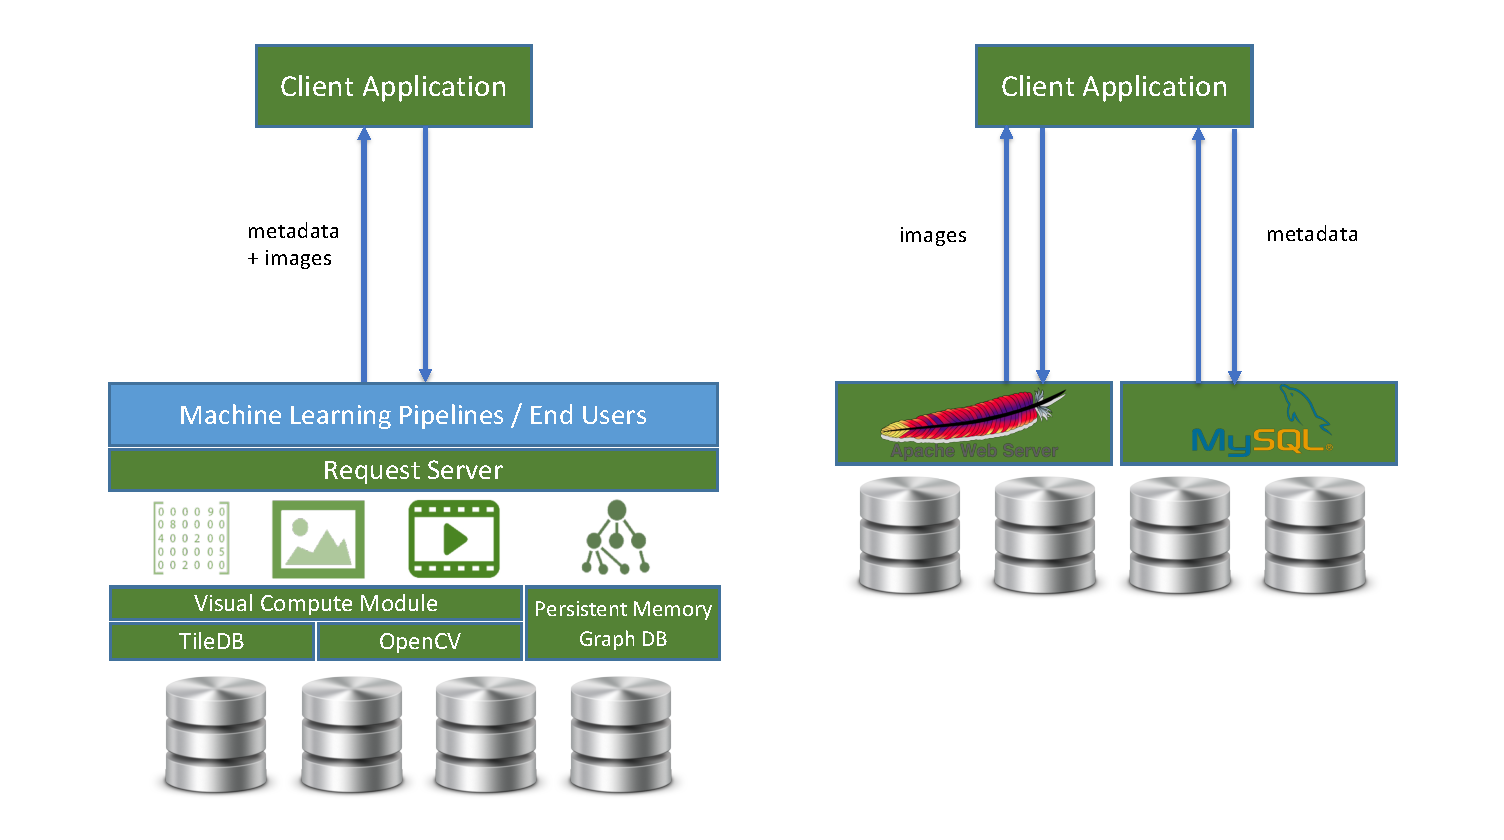
\includegraphics[width=\textwidth]{figures/comparison_system}
\caption{Comparison Systems}
\label{fig:systems}
\end{figure*}

We built VDMS and MySQL databases using the YFCC100M dataset with
incremental sample sizes 100k, 500k, 1M, 5M, 10M, 50M, and 100M.
For each dataset size, we created a PMGD graph from the YFCC100m metadata,
the YFCC100m autotags associated with each metadata identifier,
and a list of 1,570 autotags using 100 concurrent VDMS Python clients.
With simple queries, we insert 1,570 nodes for the autotags and
insert nodes for the YFCC media objects with the appropriate metadata.
Adding the autotag confidence scores is a recursive process and
requires more complex queries than adding the previous nodes.
For each metadata identifier in autotags, the query must find
the associated metadata node and a tag node for an autotag listed
for the identifier.
A connection between the two nodes is created with
the confidence score as a property.
The number of metadata nodes are dependent on the database
size and the connections are responsible for 90\% of the elements
in each database as shown in Table~\ref{table:vdmsnodes}.
It is important to note that the metadata identifier, autotags,
and longitude/latitude coordinates are set as indexes of the
database to allow faster retrieval of the metadata.

\begin{table}[h]
\caption{Nodes in VDMS database}
\centering
\begin{tabular}{c c c c}
\hline\hline
Database Size & Connections & Images & Autotags\\
\hline
100k & 848,432      & 100,000     & 1,570\\
500k & 4,249,500    & 500,000     & 1,570\\
1M   & 8,503,045    & 1,000,000   & 1,570\\
5M   & 42,505,478   & 5,000,000   & 1,570\\
10M  & 85,040,404   & 10,000,000  & 1,570\\
50M  & 425,162,070  & 50,000,000  & 1,570\\
100M & 895,572,430  & 99,205,984  & 1,570\\
\hline
\end{tabular}
\label{table:vdmsnodes}
\end{table}

Alternatively, each MySQL database is created from the same data using three
tables: taglist, metadata, and autotags.
By default, MySQL accounts for thread concurrency when processing requests
but we increased the buffer pool size to handle the large amounts
of data to avoid locking ~\cite{mysql}.
Using a Python client and simple queries, the taglist table is
read from the list of tags with an auto-incremented tagid as an
index and the metadata table is read from the YFCC100m metadata
using the identifier as an index.
The autotags table contains the generated autotags and confidence
scores for metadata entries of the metadata table.
To generate the table, we split the autotags data for each database
by the metadata identifier and autotag into new files.
The new files are read into the respective autotags table
with the metadata identifier and tagid as indexes.

\begin{table}[h]
\caption{Rows in MySQL database}
\centering
\begin{tabular}{c c c c}
\hline\hline
 & \multicolumn{3}{c}{Table}\\
\cline{2-4}
Database Size & Autotags & MetaData & Tag List\\
\hline
100k & 848,912     & 100,000    & 1,570\\
500k & 4,241,200   & 498,707    & 1,570\\
1M   & 8,508,380   & 1,000,000  & 1,570\\
5M   & 42,425,905  & 4,987,379  & 1,570\\
10M  & 85,095,265  & 10,000,000 & 1,570\\
50M  & 425,446,208 & 50,000,000 & 1,570\\
100M & 896,002,496 & 99,206,564 & 1,570\\
\hline
\end{tabular}
\label{table:mysqltables}
\end{table}

\begin{figure}[]
\centering
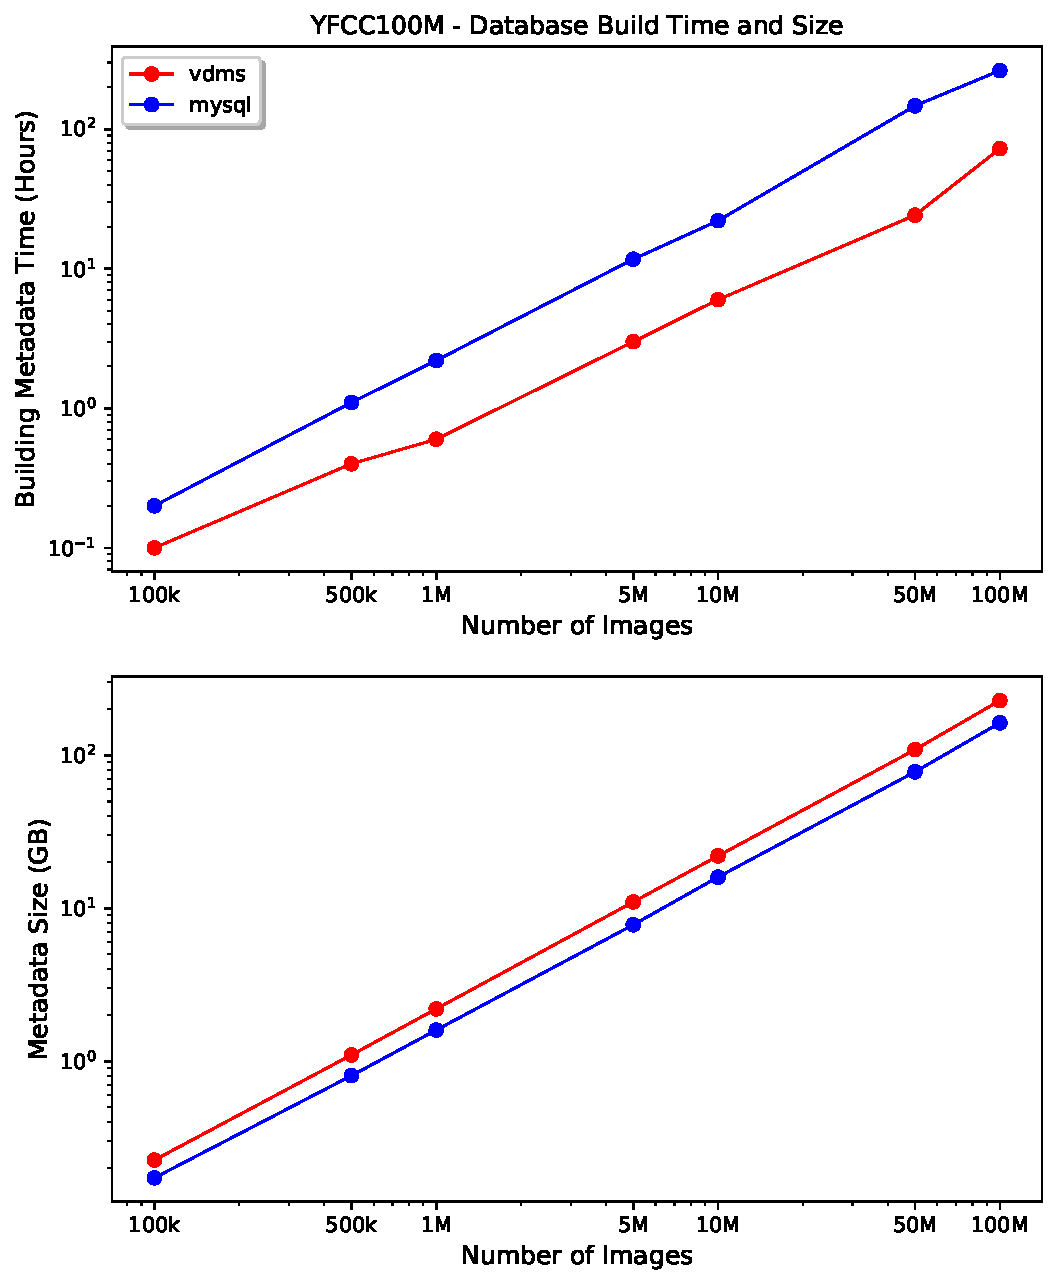
\includegraphics[width=\columnwidth]{figures/db_time_size}
\caption{Time (in hours) to build and size (in GB) of MySQL and VDMS databases}
\label{fig:db_time_size}
\end{figure}

The VDMS and MySQL databases have comparable number of elements as shown
in Table~\ref{table:vdmsnodes} and ~\ref{table:mysqltables} but
VDMS outperforms MySQL in build speed.
Figure~\ref{fig:db_time_size} illustrates how VDMS can build
databases faster than MySQL as the database size grows.
A key difference in ingestion times is the low-level implementation of
how MySQL reads data from the files and saves them to the tables
versus VDMS ability to add components concurrently.
In comparison, on average, it took MySQL 3.72x hours longer to build
each database than VDMS.
For example, to build the 100M database, MySQL took 263 hours
while VDMS only needed 72.5 hours.
This is a difference of over 7 days of processing data with
VDMS missing less than 0.001\% images and 0.048\% connections
from the entire dataset.
Alternatively, VDMS requires more storage, shown in
Figure~\ref{fig:db_time_size}, to store relationship information
about each node/connection.
This may become a factor if storage is a limitation but for the YFCC databases,
VDMS required 30-41\% more storage than MySQL.

% \begin{tabular}{c c c c c}
% \hline\hline
%  & \multicolumn{2}{c}{Building Metadata Time} & \multicolumn{2}{c}{Metadata Size}\\
% \cline{2-3} \cline{4-5}%\hline
% Database Size & MySQL & VDMD & MySQL & VDMS\\
% \hline
% 100k & 0.2   & 0.1  & 0.173 & 0.226\\
% 500k & 1.1   & 0.4  & 0.805 & 1.1\\
% 1M   & 2.2   & 0.6  & 1.6   & 2.2\\
% 5M   & 11.7  & 3.0  & 7.8   & 11\\
% 10M  & 22.1  & 6.0  & 16    & 22\\
% 50M  & 147.1 & 24.2 & 78    & 109\\
% 100M & 263.0 & 72.5 & 163   & 228\\
% \hline
% \end{tabular}
% \label{table:metadata}
% \end{table*}

\subsection{Images + Metadata}

\textbf{\textit{Explanation of the evaluation and description of some of the queries.}}

To evaluate the access to metadata and images, we use the following four queries:
\begin{enumerate}
\item {\bf {\em 1tag}}: Find metadata/images of alligator.
\item {\bf {\em 1tag\_resize}}: Find metadata/images of alligator and resize to 224x224.
\item {\bf {\em 1tag\_resize\_geo}}: Find metadata/images of alligator, resize to 224x224, and in a particular geolocation (20 degrees radius).
\item {\bf {\em 2tag\_resize}}: Find metadata/images of BOTH alligator and lake and resize to 224x224.
\end{enumerate}

\begin{figure}[]
\centering
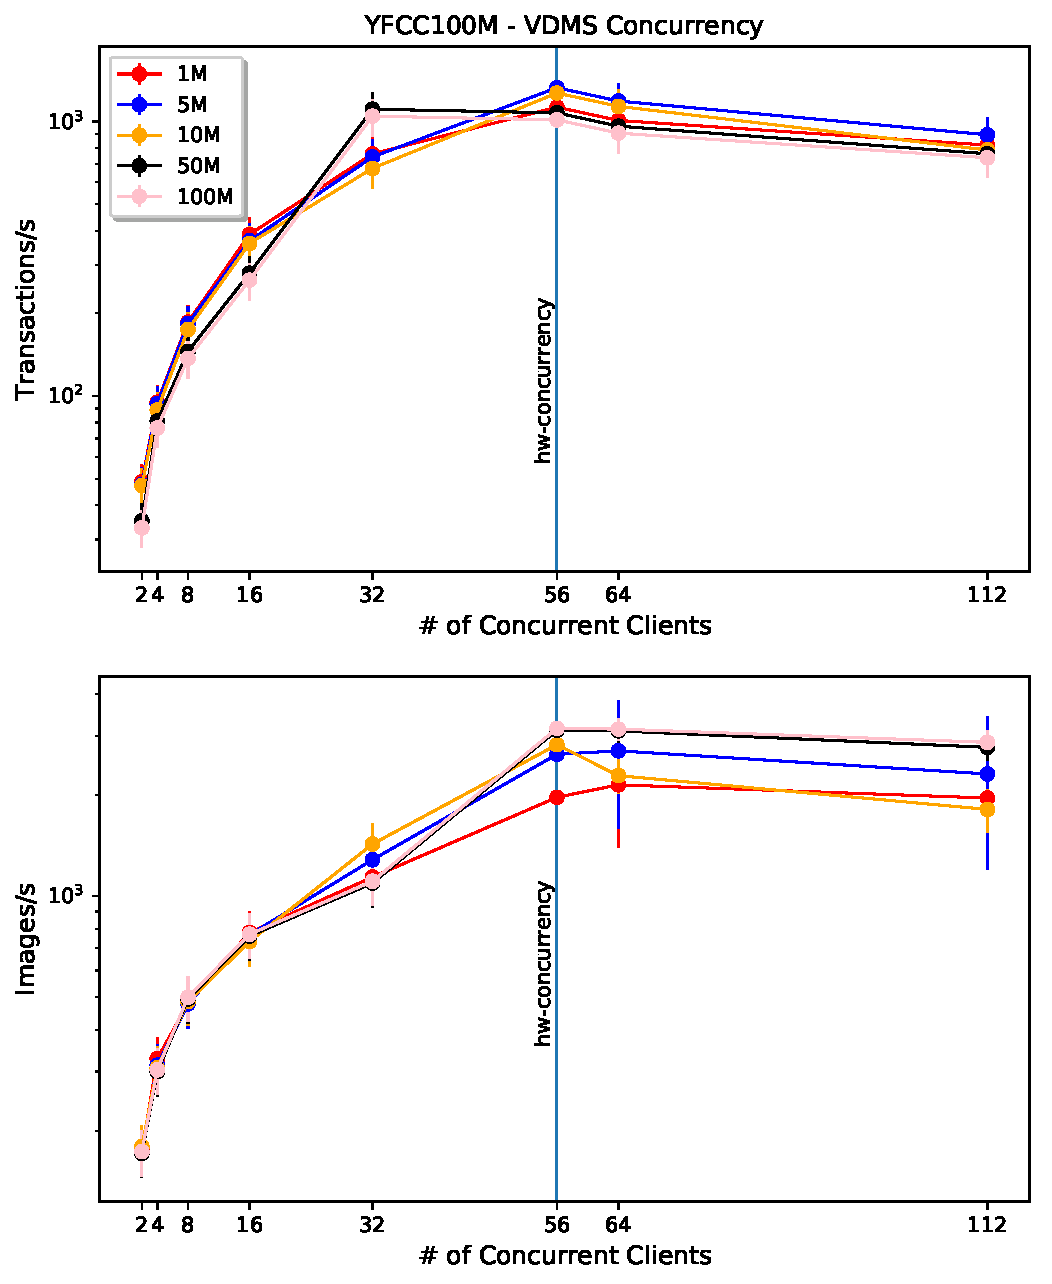
\includegraphics[width=\columnwidth]{figures/concurrency_vdms}
\caption{Concurrency Analysis - VDMS}
\label{fig:concurrency_vdms}
\end{figure}

\begin{figure}[t!]
\centering
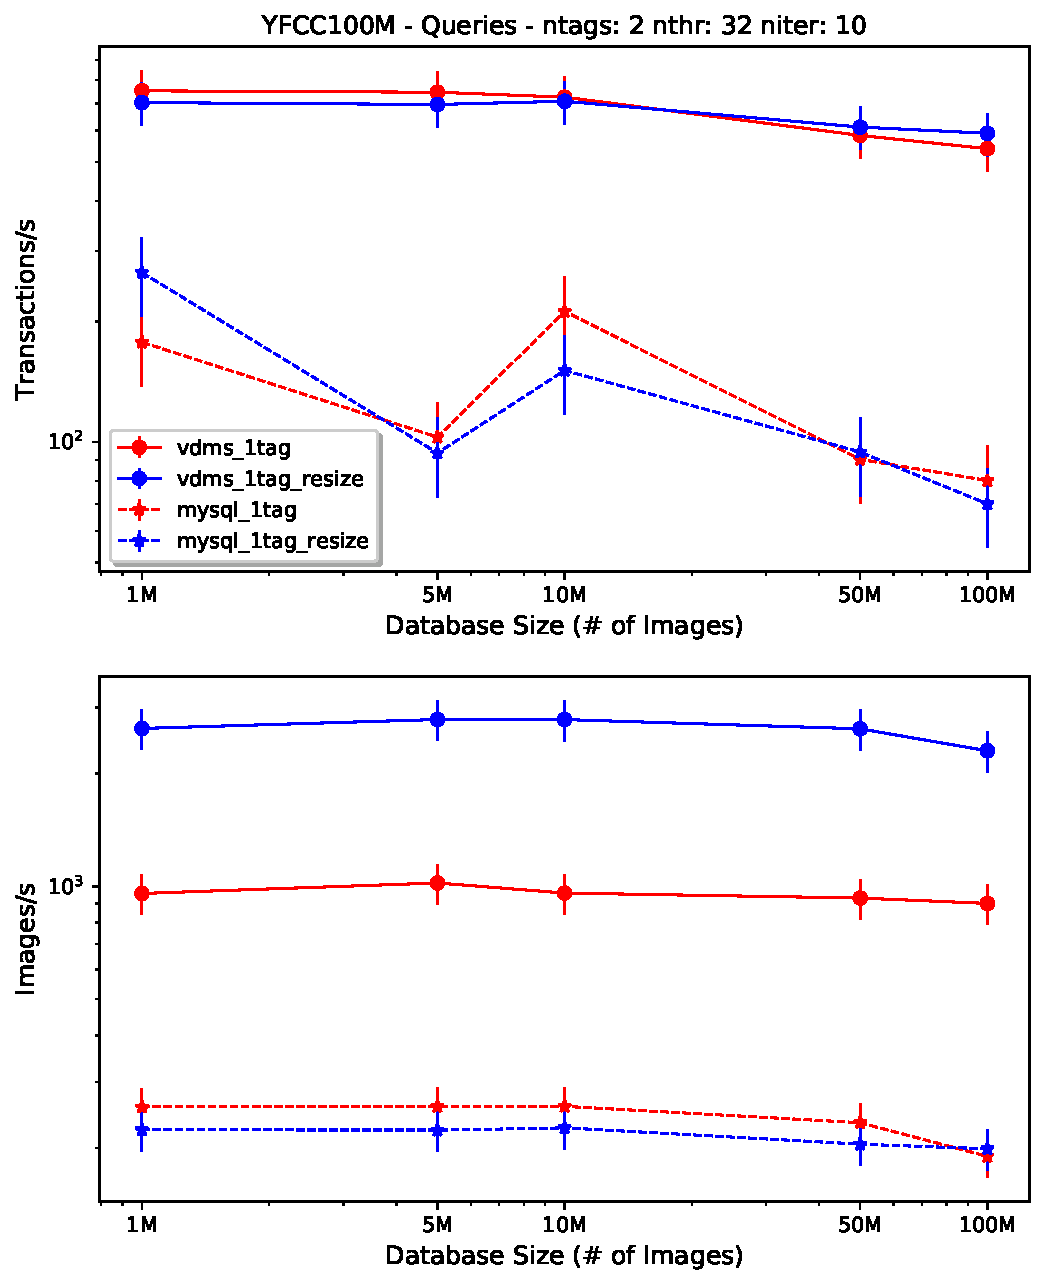
\includegraphics[width=\columnwidth]{figures/queries_throughput_32}
\caption{Queries - Throughput - 32 Clients}
\label{fig:q_throughput_32}
\end{figure}

\begin{figure}[t!]
\centering
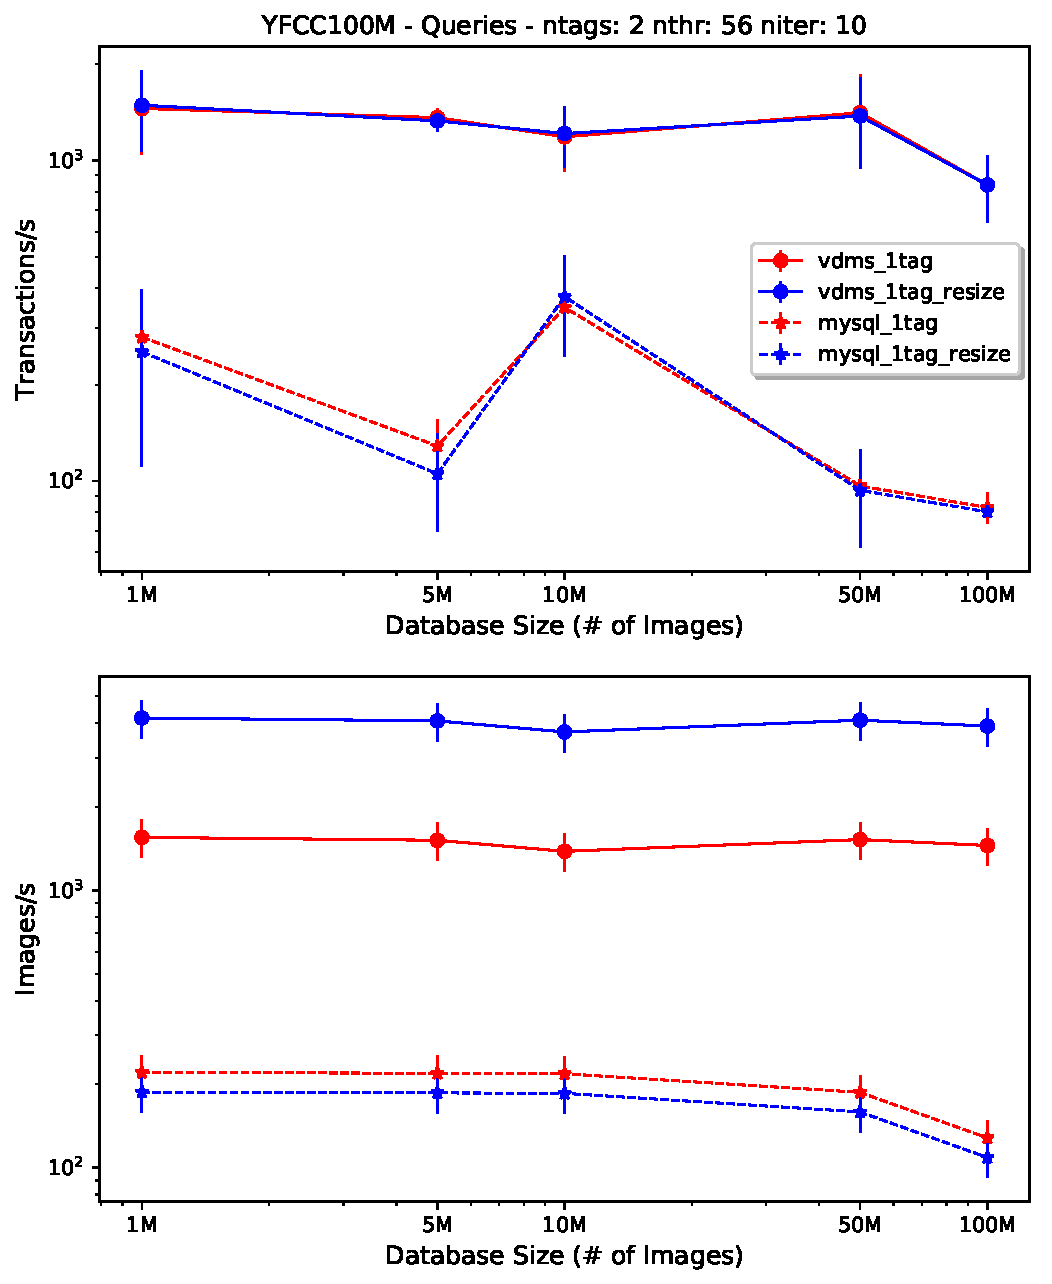
\includegraphics[width=\columnwidth]{figures/queries_throughput_56}
\caption{Queries - Throughput - 56 Clients}
\label{fig:q_throughput_56}
\end{figure}

An image and metadata search on the YFCC100M databases are very extensive
and would benefit from multithreading to process queries simultaneously.
Figure~\ref{fig:concurrency_vdms} illustrates a concurrency analysis for
the \textit{1tag} query using VDMS to investigate the number of
concurrent clients to use for the per-query performance analysis.
This figure shows the metadata performance plateaus at 32 clients and
the image performance at 56 clients for a simple query.
To further investigate, Figure~\ref{fig:q_throughput_32} and
Figure~\ref{fig:q_throughput_56} illustrate the throughput performance
for the \textit{1tag} and \textit{1tag\_resize} queries for 32 and 56 clients,
respectively.
On the 56-client experiment, a 10x difference occurs between VDMS and
MySQL in metadata throughput while 32 clients is similar but not as high.
The overall performance for both MySQL and VDMS is better with 56 clients;
therefore, we used this value for our per-query analysis.


\begin{figure}[]
\centering
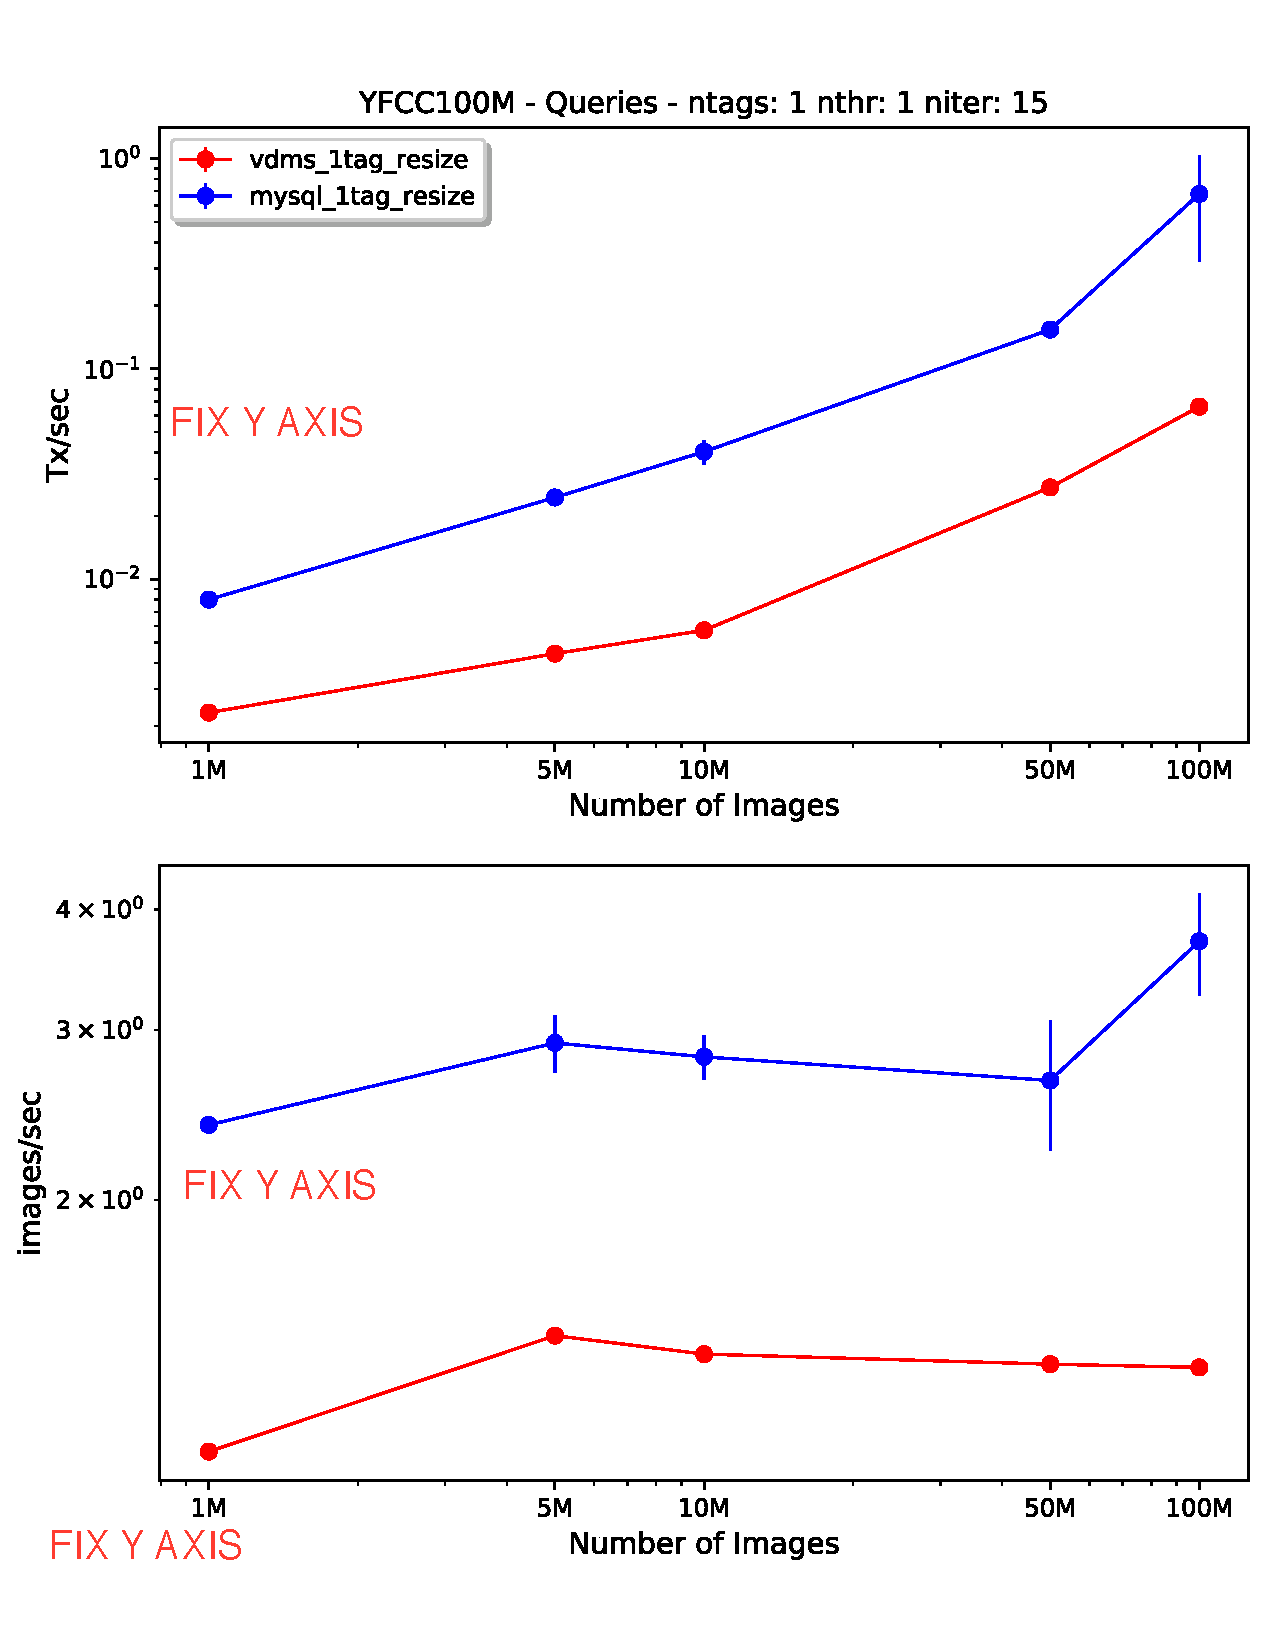
\includegraphics[width=\columnwidth]{figures/q1_latency}
\caption{Query 1 - Latency}
\label{fig:q1_latency}
\end{figure}


\subsection{Videos}

\textbf{\textit{Explanation of the video queries and comparison.
Explain concurrency.}}

\begin{figure*}[]
\centering
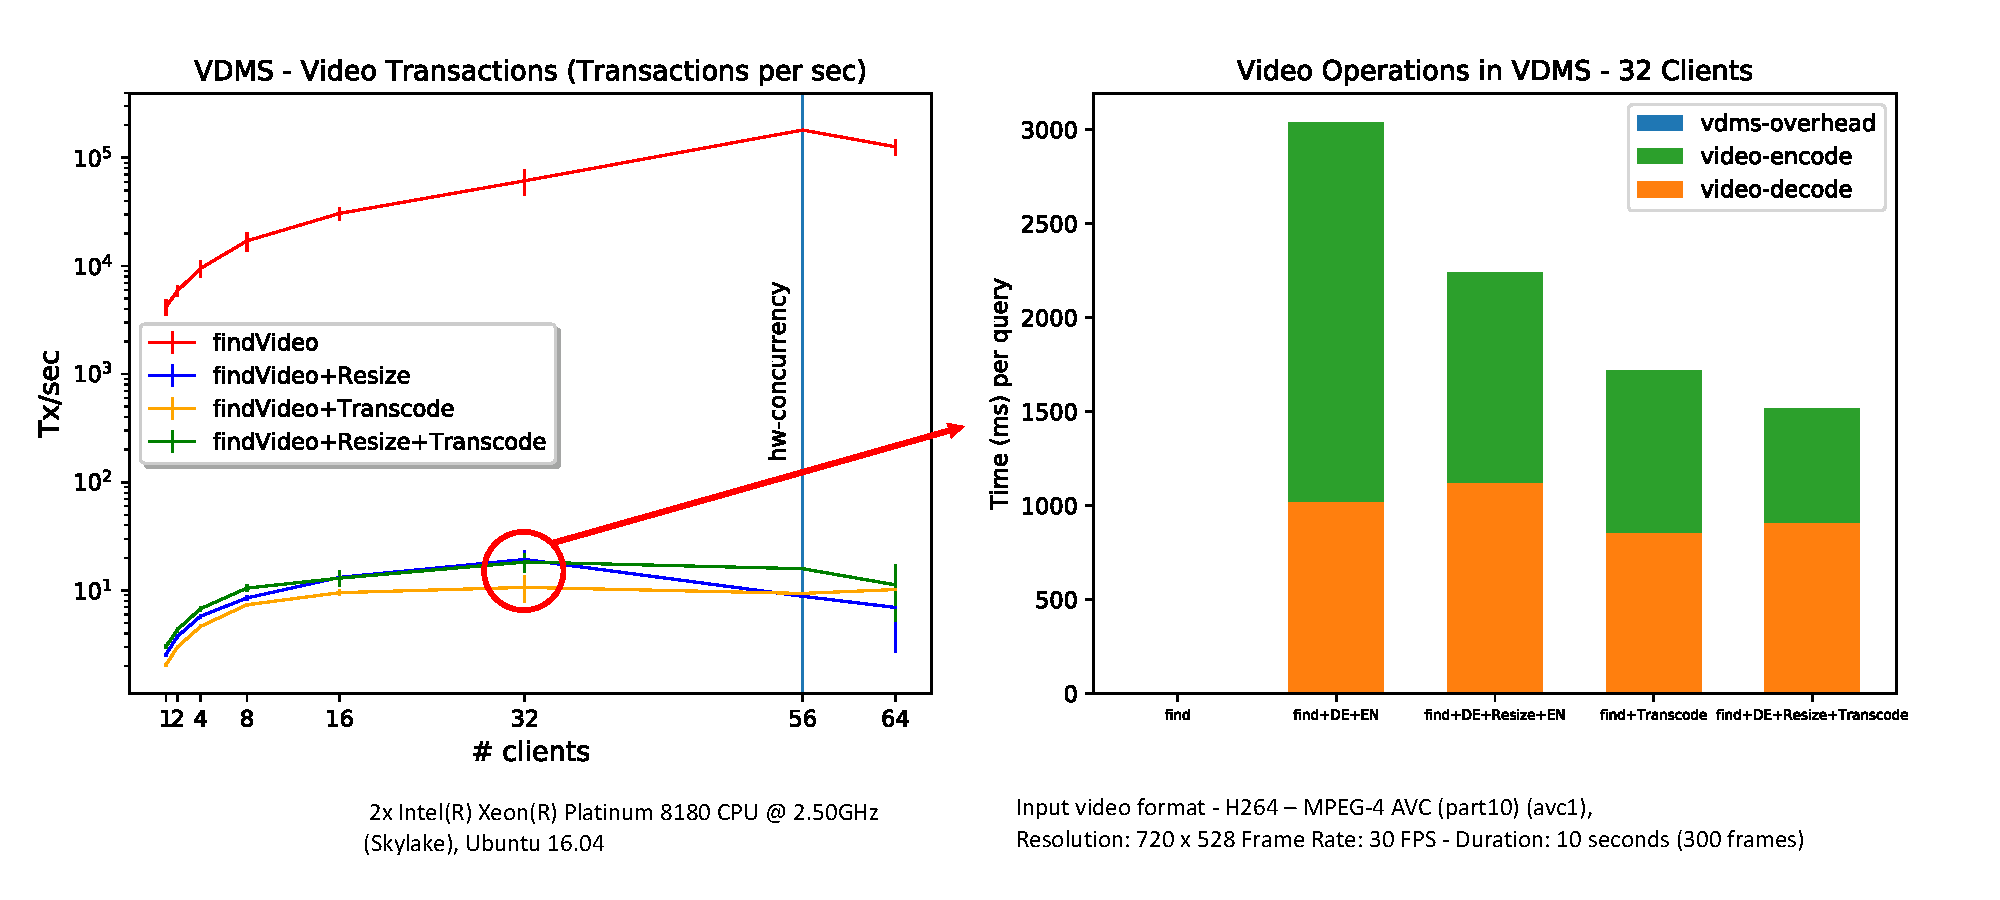
\includegraphics[width=\textwidth]{figures/video_overhead}
\caption{Concurrency and Overhead}
\label{fig:video}
\end{figure*}

\subsection{Feature Vectors}

Another key differentiating factor of VDMS is that it allows the creation of
indexes for high-dimensional feature vectors and the insertion of
these feature vectors associated with entities or visual objects.
Feature vectors are intermediate results of various machine
learning or computer vision algorithms when run on visual data.
These vectors can be labeled and classified to build search indexes,
and there are many in-memory libraries that are designed for
this task~\cite{flann, faiss}.
Using the VDMS API, users can manage feature vector indexes,
query previously inserted elements (images),
run a k-nearest neighbor search (knn) and express relationships
between existing images or feature vectors and
the newly inserted feature vectors.
By natively supporting feature vectors and knn,
VDMS allows out-of-the-box classification
functionalities for many applications.

% Figure~\ref{fig:features} shows an example of how this functionality
% can be integrated in a medical imaging analytics pipeline:
% (1) A feature vector is extracted from an bounding
% box in a brain image and labeled;
% (2) the feature vector is inserted together
% with all the associated metadata (type of cancer, for example)
% and a link to the original image.
% (3) A new feature vector is extracted from a new image,
% (4) a query to VDMS is issued to classify that feature vector based on the
% indexed features in VDMS, and
% (5) VDMS can respond to the query with the label
% associated to that feature vector.
% Note that, even if the example is based on the medical images used for the
% performance evaluation, this methodology is applicable in many other contexts
% and use cases, such as face detection and matching.
% More details about the JSON API for this functionality can be found on
% our Github wiki page.


\textbf{\textit{Explain different engines supported, and how the features vectors
were ingested and handled.}}

\begin{figure*}[]
\centering
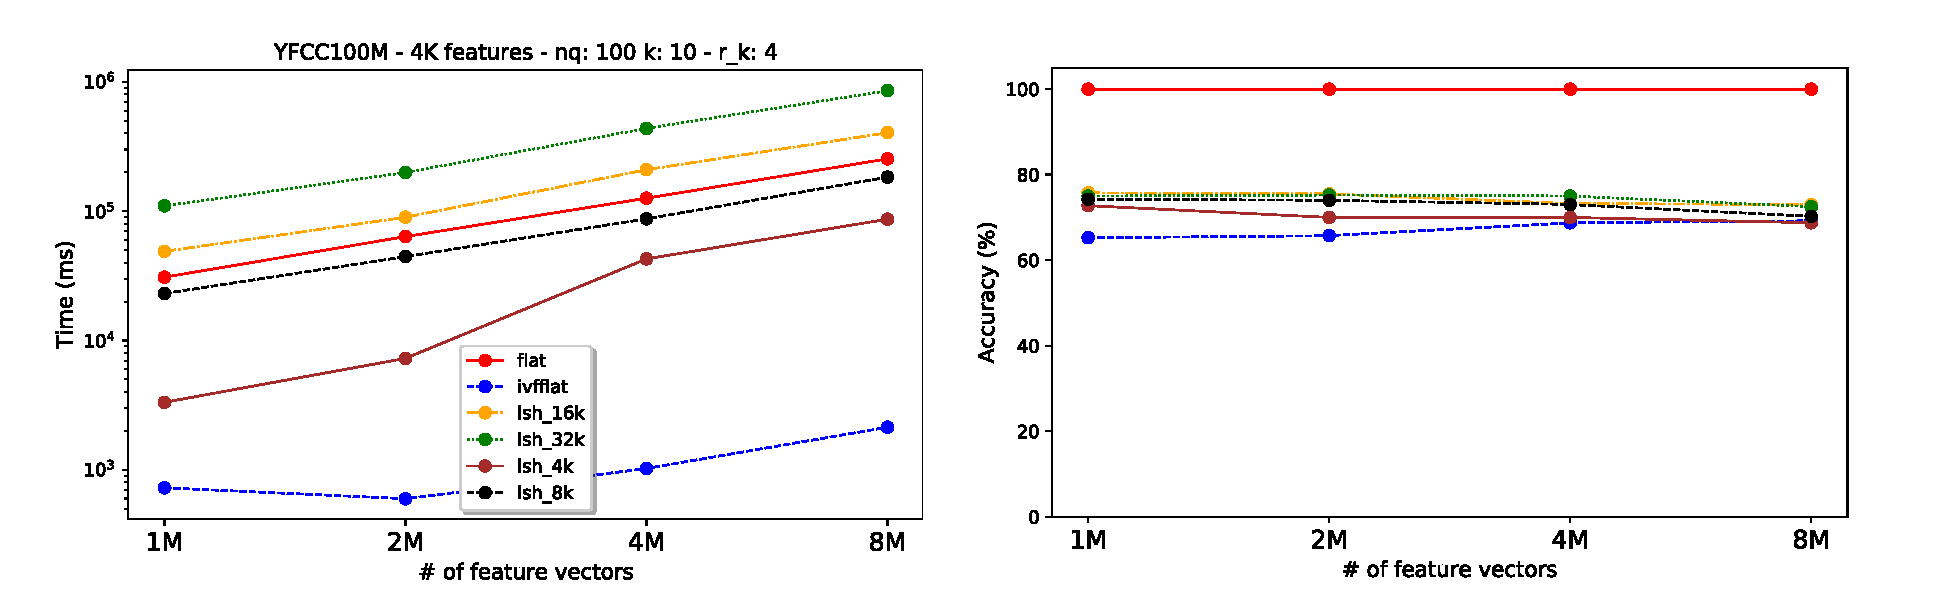
\includegraphics[width=\textwidth]{figures/features_alternatives}
\caption{Feature Vector Evaluation}
\label{fig:features_eval}
\end{figure*}

\begin{figure*}[]
\centering
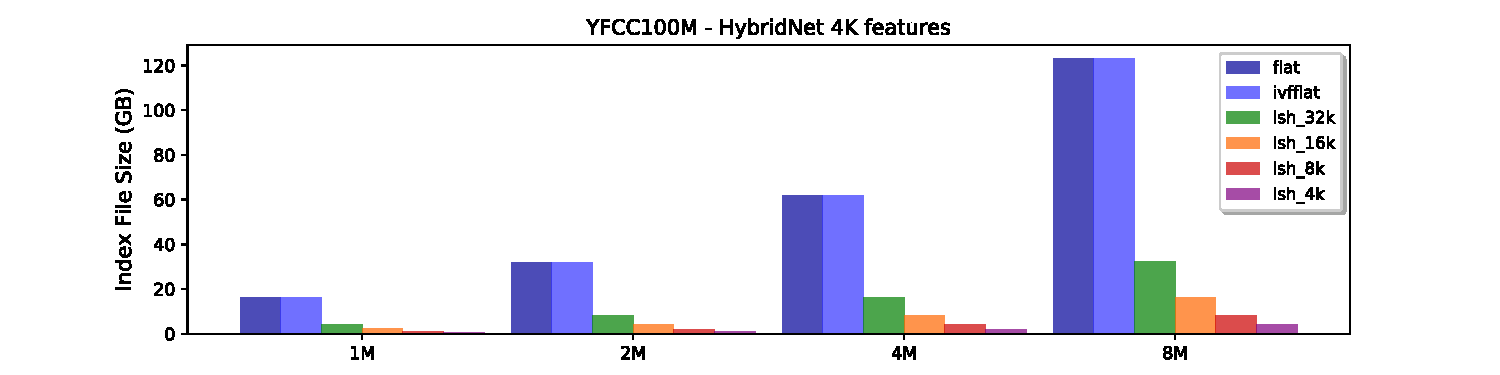
\includegraphics[width=\textwidth]{figures/features_disksize}
\caption{Feature Collection Size in Disk}
\label{fig:features_size_does_matter}
\end{figure*}
